\documentclass[a4paper,10pt]{article}
\usepackage[T1]{fontenc}
\usepackage[utf8]{inputenc}
\usepackage{amsmath,mathrsfs,bm}
\usepackage{color}
\usepackage{cleveref}
\usepackage{graphicx}
\usepackage{fullpage}
\usepackage{natbib}
\newcommand{\jb}[1]{{\color{blue} (#1)} }
\newcommand{\gc}[1]{{\color{red} #1}}
\definecolor{orange}{rgb}{1,0.5,0}
\newcommand{\kl}[1]{{\color{orange} #1}}
\newcommand{\crefrangeconjunction}{--}
\begin{document}

\title{Convergence notes}

\author{
%Jeremy J. Berg$^{1,2}$, Joseph K. Pickrell$^{3}$, and Graham Coop$^{1,2}$ \\
$^1$ Center for Population Biology, University of California, Davis.\\
$^2$ Department of Evolution and Ecology, University of California, Davis\\
$^3$ New York Genome Center\\
\small To whom correspondence should be addressed: \texttt{jjberg@ucdavis.edu, gmcoop@ucdavis.edu}\\
}

\maketitle

Evolution (journal) has a commentary section, seems like something like that could work.
%%http://onlinelibrary.wiley.com/journal/10.1111/(ISSN)1558-5646/homepage/ForAuthors.html

%Perspectives express new points of view or interpretations based on a scholarly review research. They must go beyond the works being reviewed by proposing new directions, new syntheses, and/or resolutions to old questions. Perspectives are normally solicited; however, authors may submit proposals to the Editorial Office: evoedoffice@wiley.com.
%Commentaries are invited, short essays by evolutionary biologists on any topic they believe merits discussion. Authors may submit proposals to the Editorial Office: evoedoffice@wiley.com.
%Manuscripts should be as concise as possible, consistent with clarity. For Original Articles and Perspectives, the usual limit is 7500 words of text, excluding tables, figure captions and literature cited. For the other article types, the usual limit is 4500 words.


``Convergent evolution is phenotypic similarity that is independently
derived in two or more lineages'' (Losos), definition includes both
convergence and parallelism. 

Why are we impressed by convergent evolution? Well it's because we get
to see selection act repeatedly to shape new mutations and standing
variation into adaptations in similar ways. This is particularly
impressive when we see convergence to a particular environment. Convergence helps us build
evidence that the phenotype is an adaptation, and form evidence that
adaptation is `for' increasing survival/fitness in particular
environment. 

How much do we say about genetic drift as a source of apparent convergence (and/or release from constraint).

Two distinct, but related questions, can we say that a phenotype/variant has been under selection. How many distinct instances of selection have there been. 
Related Q: as the more independent instances, the more evidence we have that it's
selected being selected.  

\paragraph{Formalizing the overlap in selection, in terms of selective
births/deaths}
When can we say that selection has been convergent in among populations?
Can we formalize this Q by thinking about the overlap in selective
deaths/births underlying the adaptative evolution of a particular trait, allele, or set of alleles within a population?


Haldane substitution load Haldane (1957), Crow 1968.
%%Crow chapter: http://link.springer.com/chapter/10.1007%2F978-3-642-46244-3_5#page-1
%% MS on solution to load paradox: http://www.nature.com/nature/journal/v219/n5159/pdf/2191114a0.pdf
%%Felsenstein: https://www.jstor.org/stable/2459384?seq=1#page_scan_tab_contents

Take care to

One locus:\\
The selective load (L) for directional selection (where fitest homozy
has selection coeff $s$) move an allele from frequency $x_1$ to $x_2$
in $t_1$ to $t_2$ generations is
\begin{align}
L &= \sum_{t=t_1}^{t_2} s(1-x_t) \\
&\approx \int_{t_1}^{t_2}  s(1-x_t) dt
\end{align}
The number of selective deaths, in a population size of $N$, is
$NL$. Assuming an additive model ($dx/dt = (s/2)x(1-x)$) 
\begin{align}
L &= \int_{t_1}^{t_2}  s(1-x_t) dt\\
&= 2  \int_{x_1}^{x_2}  \frac{1}{x} dx\\
& = 2 \log(x_2/x_1) 
\end{align}
So if the ancestral population goes from frequency $x_1$ to $x_2$, and
the descendant populations ($1$ and $2$) move this to $x_3^{(1)}$ and
$x_3^{(2)}$, then their shared deaths are $2N\log(x_2/x_1)$ and separate
deaths are $2N\log(x_3^{(1)}/x_2)$ and
$2N\log(x_3^{(2)}/x_2)$. The fraction of shared deaths would be ratio
\begin{equation}
\frac{\log(x_2/x_1)}{\log(x_3^{1}/x_1)}~~~\textrm{and}~~~\frac{\log(x_2/x_1)}{\log(x_3^{2}/x_1)}
\end{equation}
Interestingly this is mostly determined by deaths when the
allele when it is rare (wonder if this means HH will be informative).\\

Phenotype:\\
The response to selection, for a phenotype with heritability $h^2$ and
phenotypic variance $V_p$, is 
\begin{align}
R = h^2 i(p) \sqrt{V_p}
\end{align}
where $i(p)=S/sqrt{V_p}$, $i(p)$ is the selection intensity. So if the
population achieves a phenotype shift $R_T$ in $T$ generations, then
the implied selection intensity per generation is 
\begin{equation}
i(p) = \frac{R_T}{h^2 T \sqrt{V_p}}
\end{equation}  
Under trunctation selection (Lande says it the form of selection that
implies weakest selection) we can obtain the fraction ($p$) of individuals
who were parents from $i(p)$, but this isn't a nice simple
expression. Perhaps just talking about fraction of phenotypic change would be
enough, and point out that this is linked to the intensity of
selection. 

\paragraph{Why is this easier when we have changes polarized on a phylogeny?}

Why is this question easier when we have a resolved phylogeny with
no-incomplete lineage sorting (is this 2nd thing needed).
Well in that case the selective births and deaths are clearly
independent. E.g. the individuals who lived/died, due to differential
predation pressure, to drive the adaptation of light coloured fur in
arctic foxes and hares were clearly different sets of individuals
(being foxes and hares respectively). 

%Useful bib of convergence
%http://www.oxfordbibliographies.com/view/document/obo-9780199941728/obo-9780199941728-0038.xml
%https://www.jstor.org/stable/pdf/2992218.pdf 

%%felsenstein on comparative method within species
%%http://evolution.gs.washington.edu/papers/spectrum/spectrum.pdf

If we have a tree of drift (w. no gene flow), seeing non-sisters sharing an selective
event can be ``enough''. E.g. if both populations show a sweep (A \& C), not
shared with sisters (B \& D), then we have evidence that selection has occurred
in both pops independently. 

\paragraph{What do we mean, or can we say about, convergence when we only see the selected allele}


\begin{figure}
	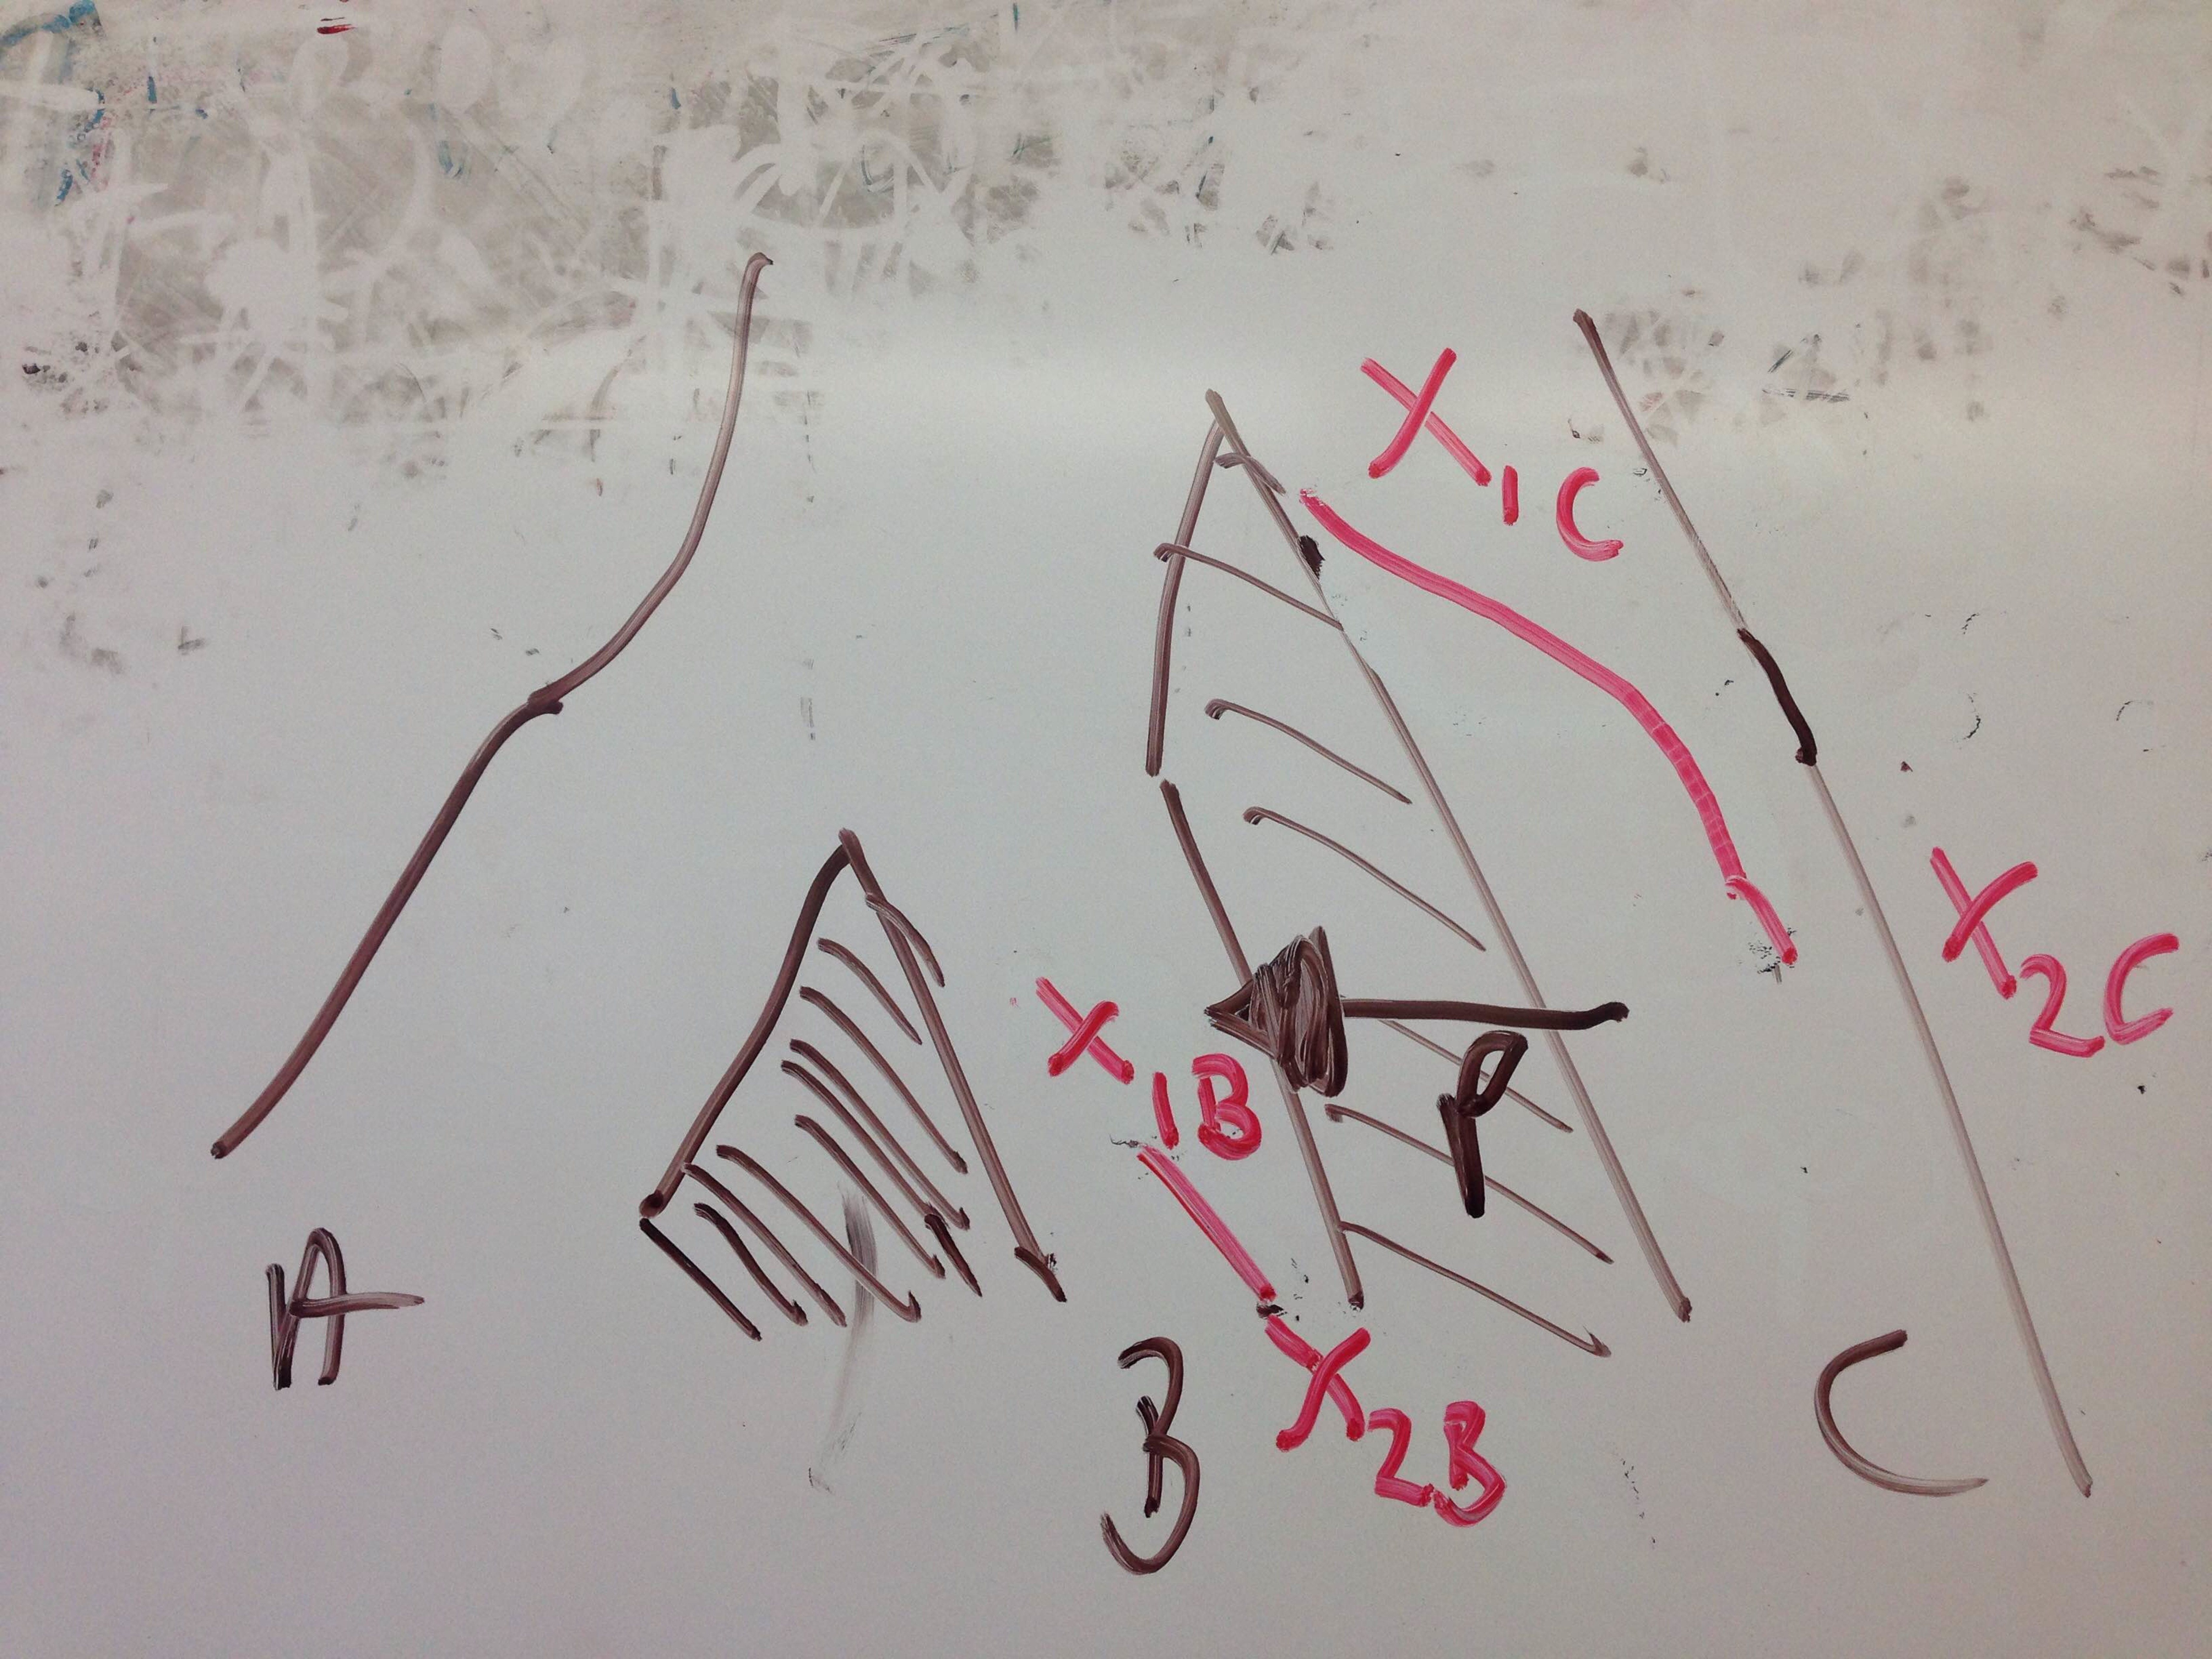
\includegraphics[width = 0.4\textwidth]{Figures/single_allele_admixture}
	\caption{BLAH}
	\label{fig:admix-graph}
\end{figure}
Consider the case, showin in Figure \ref{fig:admix-graph}. The selected allele has changed frequency in
population C, and there is gene flow from C into B (w. admixture
prop. $p$), but not into $A$. The question is, is how much convergence
has occurred in popualtion $B$?  
Assume first that allele is absent in
$A$ and was absent in $B$ prior to admixture.  The change in $C$ is
from $x_{1C}$ to $x_{2C}$. Assume that
$x_{2C}$ was the frequency when admixture occurred, an assumption conservative
against finding convergence. Then $x_{1B}$, the frequency immediately
following admixture is $pX_{2C}$. Then the selective deaths in
population $C$ and $B$ are
\begin{equation} 
2N\log(x_{2C}/x_{1C})~~~\textrm{and}~~~2N\log(x_{2B}/px_{2C})
\end{equation}
So most of the selective death will have been in population $C$ when
$px_{2C} \gg x_{1C}$. I.e. most of the action is getting the allele to
appreciable frequency, the selection after admixture is minor if the
admixture prop. is not low.\\ 

Seems like there's two questions: how much of
the selective death is shared? Is there evidence of selection at all
in population $B$ or is drift and admixture sufficient to explain the
frequency of the allele in population $B$, with selection only occurs
in population $C$.

issue of parallel clines. Could look into this. One possible eg. is
the N. American clines Drosophila clines, Link below.
%https://petrov.stanford.edu/pdfs/0117.pdf


\paragraph{What do we mean, or can we say about, convergence when we see the linked variation/sweep?}
Knowledge of variation linked to a selected site may enable us to address questions of convergence that would not be possible otherwise with certain phylogenies or only observing the selected allele.

If we observe sister populations (or populations exchanging genes) sharing a selective event, we can ask if this is convergent (i.e. shared deaths not overlapping) or if this selective event occurred in their ancestor (i.e. fraction of shared deaths greater than zero \kl{maybe come up with variable for this term?}). If the selected event is shared and the sweep is recent, we expect the regions around the selected site to be more similar than if the sweeps happened independently and are truly convergent. We can formalize this in terms of coancestry between populations.

Thinking about sister populations in Figure \ref{fig:admix-graph}, $A$ and $B$, we can define the coancestry due to both neutral processes and selection as $(f + \omega)_{ab}$ where $f_{ab}$ alone specifies the coancestry between the populations due to drift and admixture.
If the selective events occurred independently from new mutation of the beneficial allele in both populations $A$ and $B$, the coancestry between them at loci near the selected allele is simply what we expect under neutrality, $f_{ab}$.

The coancestry will increase if selection is on the same ancestral standing variant present in the ancestor of the populations, and is a function of the frequency of the standing variant, $g$ and the amount of time, $t$, once populations $A$ and $B$ have split from their ancestor before selection started. Assuming the standing variant was previously neutral or was maintained in the population at some low frequency by balancing selection,
\begin{equation} 
(f+\omega)_{ab} = y^2 \left(e^{-2rt} \left(\frac{1}{1+4Nrg}+ \frac{4Nrg}{1+4Nrg}f_{ab} \right) + (1-e^{-2rt})f_{ab} \right) + (1-y^2)f_{ab}. 
\end{equation}
where $y^2$ represents the probability of both linked lineages failing to recombine off the beneficial allele. This can be approximated as $e^{-rt_s}$ where $t_s$ is the duration of the sweep phase. This increase in coancestry, that decays with distance from the selected site, is due to the fact the region around the beneficial allele looks more similar if the variant is shared. However, as the amount of time the beneficial allele is standing independently in the sister populations before selection occurs increases, we expect this similarity to decrease as recombination is occurring independently in the populations (\kl{something tying this to idea of shared deterministic vs. stochastic events Jeremy was talking about?}).

If the selective event is shared completely (i.e. the sweep occurs in the ancestor of populations $A$ and $B$ before they split), there is a further increase in coancestry. In this case the fraction of shared deaths is 1.
\begin{equation} \label{eq: sharedS}
(f+\omega)_{ab} = y^2 + (1-y^2) f_{ab}
\end{equation}

Even if the selective event is partially shared such that selection occurs in the ancestral population (for time $t_1$) and continues independently in the daughter populations (for time $t_2$), this takes the same form as (\ref{eq: sharedS}) if $t_1 + t_2 = t_s$.
\begin{equation} \label{eq: sharedS}
\begin{split}
(f+\omega)_{ab} &= e^{-rt_2}\left(e^{-rt_1} + (1-e^{-rt_1})f_{ab}\right) + (1-e^{-rt_2})f_{ab} \\
 & = y^2 + (1-y^2) f_{ab}
 \end{split}
\end{equation}
Therefore is may not be possible to distinguish cases where fraction of shared death is greater than zero such that selective event is shared completely or partially. However, it is possible to detect if truly convergent i.e. there is no overlap in selected deaths.

Additionally, knowledge of linked variation can enable us to parse whether the increase of selected variant in population $B$ is due to drift and admixture with population $C$ alone (Figure \ref{fig:admix-graph}) or is convergence. We can estimate coancestry between $B$ and $C$, $f_{bc}$, from unlinked neutral sites that incorporate effects of drift and admixture. There will be increased coancestry around the selected site if selection is occurring in both populations. Now, 
\begin{equation} \label{eq: sharedS}
(f+\omega)_{ac} = y^2e^{-r\delta} + (1-y)f_{bc} + y(1-ye^{-r\delta})f_{cc}
\end{equation}
where $\delta$ is the delay in the sweep time between populations $B$ and $C$, a function of the strength of selection and migration rate.

\paragraph{What do we mean by convergence when we are thinking of quantitative traits?}
Should we also cover when phenotypes alone are seen? in that case using covar matrix can help in QST style analysis.
Idea of double sign test?

\paragraph{What about soft sweeps in within a population?}
Are/How are multiple alleles sweeping within a population like
convergence? 

Argument: multiple mutations conferring a single (?) adaptive
phenotype have arisen and spread at this gene. This suggests that the
gene is an `important' target for adaptation within this
population. The population has adapted via multiple changes at this
gene, when it could have used other loci. But instead selection has
independently favoured each of the alleles when they were rare in the population.

Make point that number of alleles contributing to soft-sweeps within
pop. depends on pop. scaled mutation rate and not the selection coeff.

Paraphrasing Jeremy's counter-argument: If we labeled the early/deep branches in the
spread of a single selected allele, then those lineages are
independently selected up from low frequency. Why are we less impressed by
this than when multiple mutations occur at same gene?? 

Perhaps Jeremy is correct. The fact that a single variant has swept
(say) to fixation is perhaps as interesting from the perspective of the
importance of this gene as two variants each sweeping to 50\%
frequency.  The fact that this variant sweep to 100\% (if we are
looking shortly after sweep) suggests that no equivalent change arose
at some other gene depriving it of it's advantage.

Perhaps the fact that variant(s) have swept at a population at a gene
is a statement (under a simple model of the trait) about what fraction
of the mutational target for the trait is made up of this gene. 
If sweep is due to multiple variants at a gene then you learn that
$\theta_S$ is not too small at this gene but seeing a full
hard sweep at the gene instead, perhaps conveys the same info about the fraction of the mutational target gene
wide

\paragraph{Issues about meaning of convergence and incomplete lineage sorting} 
Can we say something useful about this?
%http://www.indiana.edu/~hahnlab/Publications/HahnNakhleh2016.pdf


\paragraph{Long term signal?}
Can long term selection/drift on trait or variant, erode signal of shared
history. E.g. id stabilizing selection acts separately on a shared
trait in two (now independent populations) can we fix alternate
solutions, even though we original shared pool. Similar Q about shared
haplotypes whittled away by recom/migration. 
--One Q is do we care? 


gene conversion does similar things

\end{document}